\relatorio{Transparência no cenário político: coleta e tratamento de dados do STF}
    {
        \noindent Pesquisador: Esdras Gomes Carvalho

        \noindent Orientador: Ivar Alberto Glasherster Lange Hartmann
    }
    {O presente projeto visa auxiliar o entendimento e análise do padrão de votação dos ministros do Supremo Tribunal Federal (STF) do Brasil. Dada a relevância do judiciário e a complexidade em acessar os dados dos processos, a pesquisa concentra-se em criar um banco de dados público abrangente, compreendendo pelo menos 95\% dos processos do STF. O projeto foi executado a partir da coleta dos processos disponíveis no site do STF, concentrando esforços na computação paralela com 15 máquinas virtuais. A coleta foi concluída com um total de 2.356.676 processos coletados, e serão disponibilizados de online. O projeto repr-esenta um passo fundamental na compreensão das decisões judiciais no Brasil e promete fornecer insights sobre os fatores que influenciam as decisões dos ministros, como ideologia, influências políticas e confiança no relator.
    }
    {Supremo Tribunal Federal, Análise de Dados Judiciais, Web scrapping}


\section{Introdução (Motivação)}

A tripartição dos poderes é uma das características centrais no sistema político brasileiro, e presente em boa parte do mundo, com eleições regulares para os representantes do legislativo e do executivo. O terceiro poder, o judiciário, apresenta uma importância tão grande como os demais, entretanto, diferente dos dois primeiros os interesses e padrões de decisão não são tão claros.

Aliado a isso, os dados acerca de processos são públicos, porém de difícil acesso para realizar análises de grande porte, haja vista que a suprema corte brasileira é ímpar em relação ao número de processos anuais, como pode ser visualizado na figura \ref{fig_1}. A única suprema corte com mais processos é a Índia, porém existem 30 ministros e a população é quase sete vezes superior, ao passo que o Brasil tem apenas 11 ministros. Até então, pesquisas sobre os padrões de decisão de ministros (clustering) eram realizadas com uma pequena parcela do total. 

\begin{figure}
    \centering
    \caption{}
    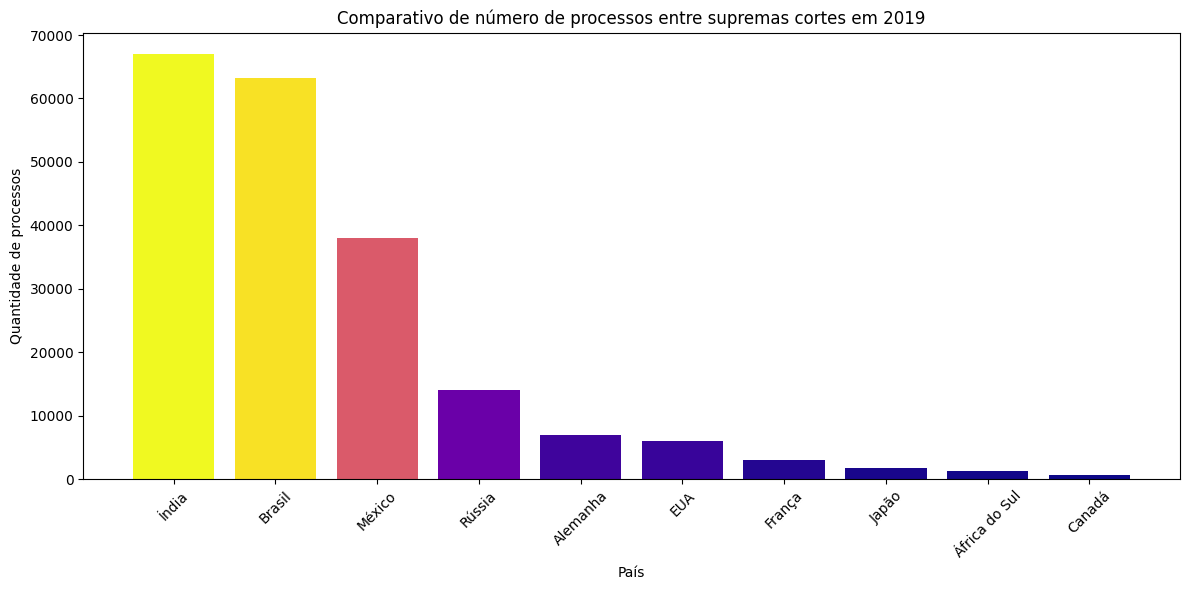
\includegraphics[width = .9\linewidth]{relatorios/stf/imagens/img2.png}
    \label{fig_1}
\end{figure}

Além disso, não há dados estruturados sobre quais foram as decisões, de modo que, a análise de como cada ministro votou se dá em um processo artesanal de leitura do texto da decisão e saber quais ministros estavam presentes à época. Isso torna uma análise geral inviável. Contudo, dado que a informação de quais ministros compunham o rol de magistrados do supremo na data da decisão esteja disponível, o texto da decisão possibilita a utilização de um algoritmo que se baseia em expressões regulares (RegEx), e tem por objetivo a classificação dos votos dos ministros em cada decisão analisada.

Nesse sentido, o presente projeto tinha como objetivo inicial responder a pergunta “Como votam os ministros do STF?”, tentando compreender se existem agrupamentos de ministros e quais os fatores que levam as suas decisões (ideologia, influências políticas, confiança no relator, etc.). O projeto focou na criação de um banco de dados público, com pelo menos 95\% dos dados dos processos do STF, presentes no site (https://portal.stf.jus.br/), sendo uma primeira etapa de 3 para responder a pergunta proposta. 

\section{Metodologia aplicada}

	Para a coleta dos dados, foi necessário seguir as seguintes etapas: levantar quais dados do processo seriam salvos, analisar a estrutura do site, estudar requisições HTTPS realizadas, criar código de web scrap, realizar testes, selecionar uma proposta de arquitetura e, por fim, a limpeza e manipulação dos dados. 

	A partir de consultas ao orientador, o levantamento dos dados relevantes para análise foi realizado. Abaixo são apresentados cada dado e uma breve descrição:
    
\begin{itemize}
    \item Classe: Denomina o tipo de processo dentre um rol que é de competência do supremo tribunal Federal, por exemplo: Arguição de Descumprimento de Preceito Fundamental, Ação Direta de Inconstitucionalidade, Habeas Corpus, Recurso Extraordinário, entre outros).
    \item Número: Apenas atribuído ao processo quando ele chega ao STF. Cada classe possui uma série de processos cujos números são ordenados de maneira sequencial. É possível que existam processos de classes diferentes com o mesmo número justamente por conta da sequência que é continuada a cada novo processo destinado àquela classe.
    \item Número único: número identificador do processo.
    \item Origem: local geográfico de origem do processo, se for no Brasil é apresentado o estado.   
    \item Relator: ministro do supremo que recebe o caso, faz as primeiras análises e resume o caso aos demais, caso o processo vá para decisão em turma ou plenário.
    \item Relator do último incidente: Define o relator da última movimentação do processo. Pode ser diferente do inicial porque nos casos em que a decisão da turma/plenário diverge do relator inicial ou há ausência deste, o  processo é distribuído para um novo relator.
    \item Partes: Interessados no processo e envolvidos diretamente na lide judicial (discussão) que tramita por meio do processo. 
    \item Andamentos: Atualiza o leitor sobre o status atual do processo e cada uma das etapas pelas quais ele passou dentro do Supremo. 
    \item Assunto: tema relacionado ao processo
    \item Número de origem: número do processo original como foi gerado no tribunal de origem, ou seja, o tribunal no qual o processo foi inicialmente protocolado e julgado. 
    \item Órgão de origem: o órgão que deu início ao processo, seja público ou privado.
    \item Tamanho físico do processo: quantidade de volumes, folhas e apensos do processo físico, se houver. 
\end{itemize}

Todas essas informações estão presentes no site do processo.
Em seguida, foi realizada uma análise da estrutura do site, bem como de quais requisições HTTP eram necessárias para coletar as informações desejadas. Com isso, foi possível a elaboração de um código, feito em python e com auxílio da biblioteca “beautifulsoup4”, para realizar a coleta das informações relevantes, caso haja uma classe e número de processo (significando que é um link com processo válido). 

Ao realizar alguns testes para verificar se as informações eram coletadas e ajustar o código, seguiu-se para a seleção de uma proposta de arquitetura. Nesse ponto, é importante ressaltar uma característica desafiadora desse projeto: o bloqueio temporário de acesso ao site. A saber, após uma série de requisições, o servidor do STF bloqueia a conexão (ligada ao número ip da máquina) como uma forma de evitar ataques de negação de serviço - uma série de acessos simultâneos intencionais que inviabilizam o acesso ao site.

Ciente do desafio, duas propostas foram arquitetadas, a primeira solução envolve a criação de uma máquina virtual (no inglês, virtual machine comumente abreviado para VM) ec2 que realiza chamadas para uma função lambda, que realiza o web scrap e salvamento dos dados no dynamoDB (banco não relacional da amazon). Essa primeira arquitetura foi aplicada na primeira coleta e a sua vantagem seria a mudança de ip de forma dinâmica, já que o aws lambda é usado em arquiteturas servless, de modo que, quando a função é chamada, uma VM com o código é criada e realiza a execução do código. Esse processo ocorre “debaixo dos panos” e permite a execução do código em máquinas diferentes a cada execução. Para a primeira coleta foram utilizadas 3 dessa arquitetura (uma VM, uma lambda e um banco dynamoDB em cada conta).

Contudo, a primeira coleta apresentou algumas falhas, elencadas a seguir: A escolha de como considerar um processo válido, que na primeira coleta era a presença de número único, contudo há processos válidos sem número único; Descobriu-se que a lambda não realiza esse processo de subir uma nova máquina a cada requisição, somente após alguns minutos (tipicamente uns 10 a 20). Desse modo, elas também sofriam com o bloqueio temporário; Além disso, um certo intervalo que continha processos válidos (do número de incidente 1 até 1465222). Devido a essas falhas e somado a questão do preço, tendo em vista que o tempo de computação numa VM ec2 é bem mais barato que o de uma lambda, uma nova arquitetura foi proposta para a segunda coleta. 

Antes de apresentar a proposta, é válido ressaltar que foi realizado um estudo sobre a presença de processos válidos e sua relação com o número de incidentes. Esse processo se deu a partir de uma verificação de existência de processos válidos a cada 1000 números incidentes, para buscar por “buracos” na sequência, relatados pelo professor Fernando (autor da primeira coleta realizada semelhante a essa). Com isso, foi determinado um intervalo a ser buscado de 1 a 15.000 e de 1.400.000 a 6.605.876, usado na próxima coleta.

A partir disso, a segunda arquitetura foi posta em prática, que consiste em concentrar os esforços na computação paralela. A segunda proposta contém 15 VMs e 3 bancos dynamoDB e dessa vez a VM realiza o processo completo de coleta, manipulação e salvamento dos dados. Para essa segunda versão, alguns cuidados extras foram adotados, como a criação de cláusulas de erro no código, de modo que os processos que falharam tem um log escrito no arquivo “errors.txt” e a presença de um “checkpoint.txt” para saber em que ponto da coleta a máquina se encontra. Após criar o código a ser utilizado nas VMs, foi criado um service do systemd (para mais informações sobre acesse o link https://www.baeldung.com/linux/create-remove-systemd-services), para permitir que o código continuasse rodando mesmo que não esteja conectado a máquina, bem como facilitar o monitoramento. 
	
\section{Resultados}

Na primeira coleta foram levantados cerca de 1.490.986. Os valores por ano dos processos coletados são apresentados na imagem \ref{fig_2}.

\begin{figure}
    \centering
    \caption{}
    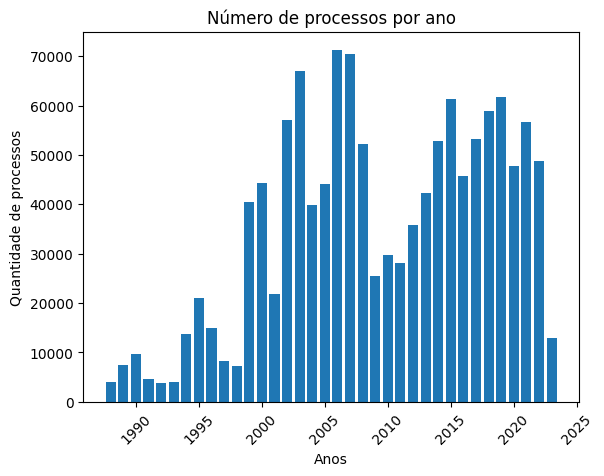
\includegraphics[width = .5\linewidth]{relatorios/stf/imagens/img1.png}
    \label{fig_2}
\end{figure}

A segunda coleta coletou 2.356.676 processos. A partir da contagem de processos que falharam chega-se à conclusão que esse valor representa cerca de 99,96\% do total de processos existentes no intervalo considerado. Os dados serão disponibilizados para acessos online, com auxilio do time de Ciência de dados do Insper, a partir da disponibilização de uma máquina virtual para hospedar os dados.  



